\section{SeqGPLVM-MSM}
\label{sec:seqgplvm}

SeqGPLVM in combination with MSM consists of three
stages: (i) a latent variable model (SeqGPLVM) that estimates a substitute for the
unmeasured confounder based on the observed treatment sequence, (ii) estimating
the propensity scores using a treatment model that conditions on both observed
covariates and the confounder substitute, and (iii) a marginal
structural model that uses the estimated propensity scores in stage two to adjust
for confounding using IPTW. It is worth mentioning that SeqGPLM can be used
in conjuction with any other estimation methods as well, such as g-computation or doubly
robust methods, but we focus on IPTW estimation of MSM for comparability with
FE-MSM.

%\hl{It seems that we dont need a first order CMM necessarily, we can have higher order CMMs as well? for now I 
%will keep it first order because that is what Hatt et al do.}

\subsection{Sequential deconfounding}

The sequential deconfounding theory proposed by 
\citeA{hattSequentialDeconfoundingCausal2024} can be seen as the sequential version of 
the multi-treatment deconfounder proposed by \citeA{wangBlessingsMultipleCauses2019}. Similarly 
to the multi-treatment deconfounder, it is based on the three key assumptions that are 
described below. 

%SeqGPLVM
%is a probabilistic 
%longitudinal latent variable 
%model. 

\begin{idassumpSG}[CMM(p): Conditional Markov Model of order p]\label{ass:SG-Marcovianity}
    A latent variable $Z$, a fixed order $p \in \mathbb{N}^*$
    and a parameter vector $\boldsymbol{\gamma} = (\gamma_1, \ldots, \gamma_T)$ exist such that the assigned treatment distribution can be 
    factorized as: 
    \begin{equation}
    p_{\boldsymbol{\gamma}}(\bar{a}_{T} \mid \bar{\mathbf{x}}_{T}, \mathbf{z}) 
    = \prod_{t=1}^T p_{\gamma_t}(a_{t} \mid a_{t-p:t-1}, \mathbf{x}_{t}, \mathbf{z}). 
    \label{eq:cmm}
    \end{equation}
    for $t<1$, $a_t$ is set to $0$ by convention. We then say that the 
    latent variable Z follows a Conditional Markov Model of order p, 
    written $Z \sim \text{CMM} (p).$
     
\end{idassumpSG}
The original version of this assumption 
in \citeA{hattSequentialDeconfoundingCausal2024} is stated only for a first-order CMM. However, 
the proof of their Theorem 1 using Preposition 7.6 in \citeA{kallenbergFoundationsModernProbability}, 
can be easily extended to higher-order CMMs as well 
(see \href{https://chatgpt.com/share/69c7c2fe-2f64-8388-8843-b0d989e7b267}{link} 
and \cite{bouchattaouiCausalDynamicVariational2025}). Hence the more general 
form of the CMM assumption is stated above. In Equation~\ref{eq:cmm},
\(\gamma = \{\gamma_0, \gamma_2, \ldots, \gamma_T\}\) are the \emph{generative} 
parameters of the treatment assignment model. Note that the conditional 
probability 
distribution at
each time point can have different parameters. 
This is cruicial to understand the SeqGPLVM architecture. 

\begin{idassumpSG}[No unmeasured single-time-point confounding]
    \label{ass:SG-No-single-time-point-confounding}
    All confounders that only affect at a single time point are observed. 
    Equivalently, any unobserved confounder influencing $A_t$ must also induce 
    dependence with at least one other treatment $A_s$ ($s\neq t$), conditional on the observed history.
\end{idassumpSG}
This assummption excludes structures such as the one in 
Figure~\ref{fig:single-time-point-confounding}. Note that, Assumption~\ref{ass:C-timeinvariant-uc} 
is not 
sufficient to exclude these single-time-point confounders since a confounder can 
be constant but its effect 
varry with time. 

\begin{figure}
    \centering
    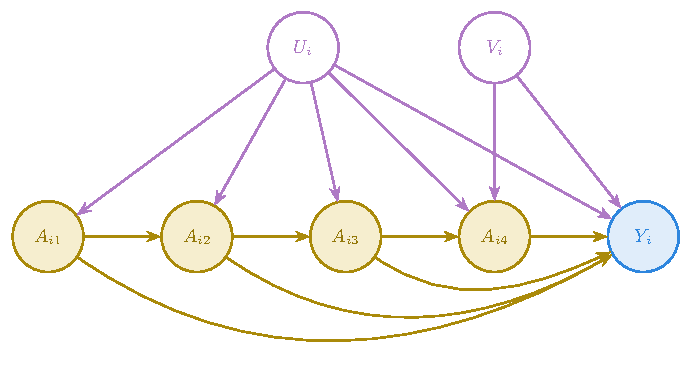
\includegraphics[width=.8\textwidth]{figures/build/single_time_point.pdf}
    \caption{Sequential deconfounder excludes unmeasured single-time-point confounders such $V_i$. }
    \label{fig:single-time-point-confounding}
\end{figure}

\begin{idassumpSG}[Consistency of the substitute confounder]
    \label{ass:SG-Consistency}
The sequential deconfounder assumes that all latent variables $Z\sim\text{CMM}(p)$ for a particular 
$p$ are pinpointed 
by a single deterministic function of treatment and observed covariates history. 
Formally, there exists a measurable function
$f$ such that
\[
p(z \mid \bar x_T, \bar a_T) = \delta_{f(\bar x_T,\bar a_T)}.
\]    
\end{idassumpSG}
Assumption~\ref{ass:SG-Consistency} implies the uniqueness of the substitute confounder. 
 This assumption is necessary since only the existance of a CMM, does not guaranty the uniqueness of the latent 
 variable \cite{damourMultiCauseApproachesCausal2019}. However, the substitute confounder is not 
 required to coincide with the true confounder $U$ or the true latent factorizer $Z$. It is sufficient 
 to estimate the substitue confounder up to some deterministic bijective 
 transformation,e.g., a linear 
 transformation.  

Under these assumptions
and the common assumptions, Theorem 1 in \citeA{hattSequentialDeconfoundingCausal2024} 
states that we obtain sequential ignorability 
conditioned on the observed covariates' history, treatment history and the
substitute confounder $Z_i$, i.e., for all $t \in \{1, \ldots, T\}$ and for all $\bar{a}_t$,
\begin{equation}
    \label{eq:seqgplvm-single-unit-seqignorability}
    Y_{i}(\bar{a}_{T}) \perp A_t \mid \bar{X}_{it}, \bar{A}_{i,t-1} ,Z_{i}.
\end{equation}
This theorem makes a bridge between the observational world and the potential outcomes world. 
More importantly, this theorem does not restrict the class of models that can be used to 
estimate the substitute confounder. It holds for any 
latent variable model that can estimate a latent variable $Z$ in a CMM of chosen order $p$.

\subsection{SeqGPLVM}


\subsection{Outcome model}
In \cite{hattSequentialDeconfoundingCausal2024}, the exact procedure for adjusting for unmeasured time-invariant confounding using SeqGPLVM is as follows:
\begin{itemize}
    \item \textbf{Stage 1: Sequential Latent Factor Model.} Fit a latent variable model to the 
    observed treatment history over time to estimate the confounder substitute $\mathbf{z}_i$ for each individual.
    \item \textbf{Stage 2: Outcome Model.} Use the estimated confounder substitutes from Stage 1 as additional covariates to adjust for confounding in the outcome model. This outcome model can be MSM, G-formula, etc.
\end{itemize}
The key idea here is that once we have estimated the confounder substitutes $Z_i$, we can 
treat them as \emph{observed-like} covariates and include them in the outcome model to adjust for 
confounding, leveraging the sequential ignorability result in equation 
\ref{eq:seqgplvm-single-unit-seqignorability-t=T}. \hl{The key selling point of this approach is 
that instead of assuming the sequential ignorability, they derive it from the CMM assumption 
and argue that CMM is a more plausible assumption in many real world settings with time-varying treatments. Although 
both this claim and the proof of theorem 1 in} \cite{hattSequentialDeconfoundingCausal2024} \hl{are subject to some critique.}

Despite the flexibility of this approach in choosing 
the outcome model, it has critical pitfalls that we will discuss in section \ref{sec:hatt-problems}. 
To avoid these issues, and since we are going to use only IPTW/MSM as our outcome model,  
in our implementation, we use the estimated propensities from the
SeqGPLVM treatment model directly in the MSM using IPTW. This choice is also conceptually closer to 
the FE-MSM method described in section \ref{sec:fe-msm}. 

If the treatment assignment mechanism follows a CMM, then the task we need to solve is to find a 
map from the joint space of the observed covariates' history and treatment history and the latent 
substitute to the 
treatment assignment at each time point. This task can be done using any latent variable model that can fit a CMM. Mathematically, we need to find functions \(f_t\) such that 
\[
f_t \colon \mathcal{Z} \times \mathcal{X}_t \times \mathcal{A}_{t-1} \rightarrow \mathcal{A}_t
\]

In SeqGPLVM, we model these functions as non-parametric functions using Gaussian processes (GPs), 
i.e., \(f_t \sim \mathcal{GP}(0, k_t(\cdot, \cdot))\) for \(t = 1, \ldots, T\), where \(k_t\) is the kernel function at time \(t\). 
The use of GPs allows for flexible modeling of complex, non-linear 
relationships between the latent confounders, observed covariates, 
and treatment assignments over time. Since the kernels are defined on the joint space of the latent substitutes and the observed history, 
we have a lot of flexibility to encode different types of interactions between these variables. For the sake 
of simplicity, we use the same kernel for all time points, but in principle, 
we can use different kernels at different time points. The inference task is then to estimate the joint posterior 
distribution of the latent confounder substitutes and the latent functions given the observed treatment history and covariates. We can write 
the joint posterior distribution as follows:
\begin{align}
p(\mathbf{Z}, \mathbf{F} \mid \mathbf{A}, \mathbf{X})
&\propto p(\mathbf{A} \mid \mathbf{F})\, p(\mathbf{F} \mid \mathbf{Z}, \mathbf{X})\, p(\mathbf{Z}\mid \mathbf{X}) \\
&= \prod_{i=1}^N \prod_{t=1}^T p(a_{i,t} \mid f_t)\, p(f_t \mid \mathbf{z}_i, \mathbf{x}_{i,t})\, p(\mathbf{z}_i)
\end{align}
where \(\mathbf{Z} = \{\mathbf{z}_1, \ldots, \mathbf{z}_N\}\) is the set of 
latent confounder substitutes for all individuals, 
\(\mathbf{F} = \{f_1, \ldots, f_T\}\) is the set of latent functions for all 
time points. 
In the last line we assume the prior distribution over the latent 
confounding substitute,  \(p(\mathbf{Z}\mid \mathbf{X}) = p(\mathbf{Z})\). 
This is the called none amortized version of the SeqGPLVM, 
where we do not condition the prior distribution of the latent 
confounder substitutes on the observed covariates. 
In principle, we can also have an amortized version where we use a 
neural network to parameterize 
this prior. More details in \ref{discussion}. We also assume that the latent confounder substitutes are distributed 
i.i.d. across individuals. 

Since the exact posterior distribution is intractable, we adopt the 
variational inference with inducing point \cite{titsiasBayesianGaussianProcess2010} for inference. 
Since the GP kernels are defined on \(\mathcal{Z} \times \mathcal{X}_t \times \mathcal{A}_{t-1}\), 
the dimensionality of the inducing points is \(|\mathcal{Z}| + |\mathcal{X}_t| + |\mathcal{A}_{t-1}|\). 
The likelihood term \(p(a_{i,t} \mid f_t)\) is dependent on the type of treatment variable. 
For instance if \(\mathcal{A_t}\in \{0,1\}\), we can use a Bernoulli likelihood, 
and if \(\mathcal{A}_t\) is continuous, we can use a Gaussian likelihood. For more 
details on the inference procedure, see \ref{sec:seqgplvm_loss}. In Fig \ref{fig:seqgplvm_architecture} we show 
the inference DAG of the SeqGPLVM.
\begin{figure}[ht]
    \centering
    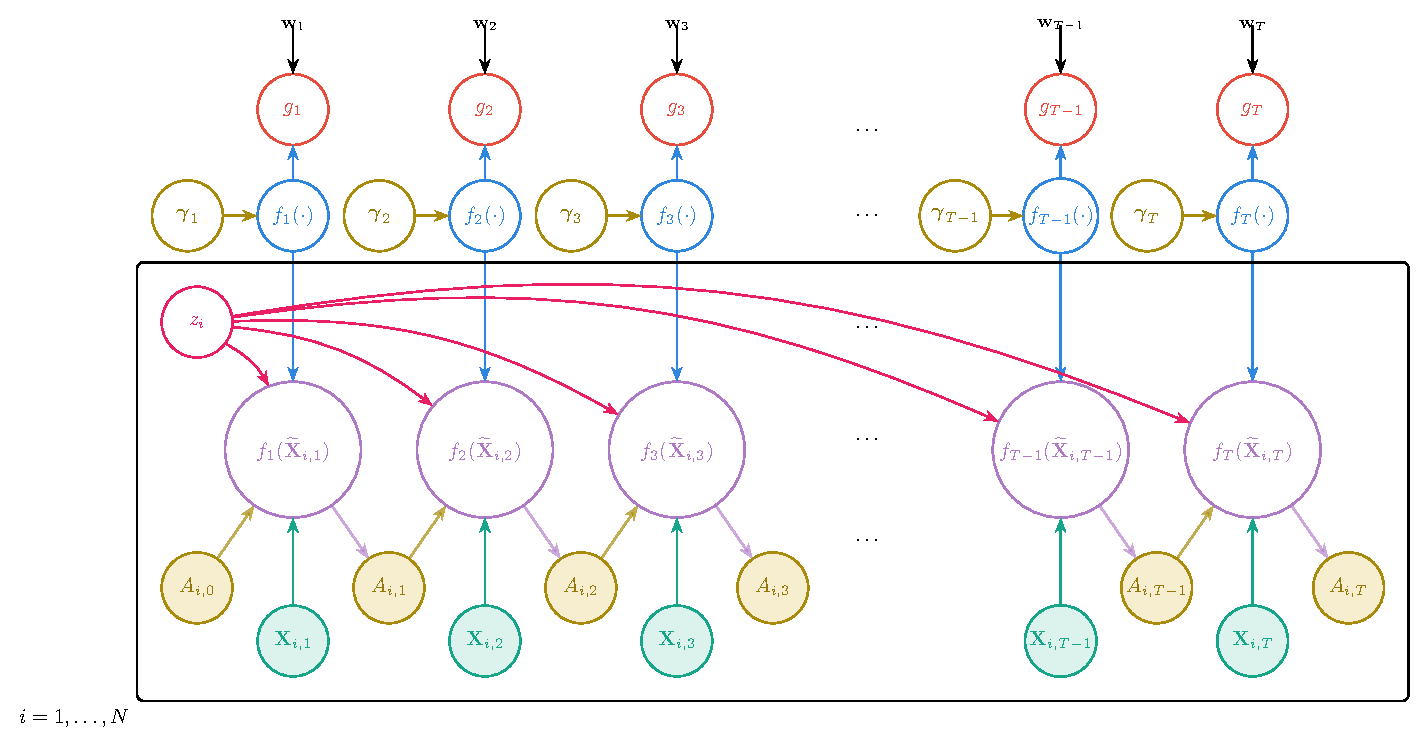
\includegraphics[width=\linewidth]{figures/build/fit_seqgplvm_dag.pdf}
    \caption{Plate diagram of the first-stage SeqGPLVM treatment model used to estimate
time-varying propensity scores. For each time point $t$, a Gaussian process
$f_t(\cdot)$ with hyperparameters $\theta_t$ maps the latent state and
observed history into the assignment probability for $A_{it}$.
The variables $u_t$ denote GP function values at inducing inputs $m_t$
(shown without nodes as they are treated as parameters).
Filled nodes indicate observed quantities and unfilled nodes latent quantities.
The outer plate indexes individuals $i = 1, \dots, N$ and the temporal structure
repeats over $t = 1, \dots, T$. The diagram represents the conditional 
assignment model underlying propensity-score estimation and does not 
impose a model on the marginal distribution of the covariate process.}
    \label{fig:seqgplvm_architecture}
\end{figure}
